\documentclass[conference]{IEEEtran}
\IEEEoverridecommandlockouts

\usepackage[T1]{fontenc}
\usepackage[utf8]{inputenc}
\usepackage{cite}
\usepackage{amsmath}
\usepackage{graphicx}
\usepackage{array}
\usepackage{tabularx}
\usepackage{booktabs}
\usepackage{textcomp}
\usepackage{xcolor}
\usepackage{xurl}
\usepackage[hidelinks]{hyperref}

\begin{document}

\title{\fontsize{20}{23}\selectfont MyoElektra: A Surface-EMG Game Controller for People with Upper-Limb Loss\vspace{-0.4\baselineskip}}

\author{\IEEEauthorblockN{Alex Smith}
\IEEEauthorblockA{Department of Electrical and Computer Engineering\\
Rice University, Houston, TX, USA\\
as636@rice.edu}}

\IEEEaftertitletext{\vspace{-1.3\baselineskip}}
\maketitle

\begin{abstract}
People with upper-limb loss have few button-free ways to use computers and games: accessible hubs require presses, and surface electromyography (sEMG) wearables are built for intact wrists and proprietary apps, not standard controllers. MyoElektra aims to read sEMG from the residual limb and present it to any computer as a standard USB gamepad that needs no drivers or host software. It pairs a SEN0240 dry-electrode sensor with a Teensy~4.1 microcontroller that filters the signal, extracts its envelope and maps contractions to controller inputs. Currently, the review of existing solutions is complete, the sensor has been selected and ordered, and the Teensy enumerates as a USB joystick and mouse that Steam recognizes without driver installation; hardcoded inputs have also steered a car in a racing game. Remaining work targets latency of at most 100~ms, at least 95\% gesture accuracy and under one false trigger per minute.
\end{abstract}

\begin{IEEEkeywords}
Electromyography, assistive technology, upper-limb amputation, human--computer interaction, USB HID, embedded signal processing.
\end{IEEEkeywords}

% ---------------------------------------------------------------------------
\section{Introduction}

Nearly every computer input device, from the mouse and keyboard to the game controller, assumes a working hand. For someone who has lost a hand or forearm, using a computer or playing a game depends on assistive hardware, and the available options differ in how they read the user's intent and where they send it.

The closest existing solutions fall into a few groups. Consumer products include adaptive switches and controller hubs such as the Xbox Adaptive Controller~\cite{xac}, and muscle-sensing wristbands such as the Mudra Link~\cite{mudra} and Meta Neural Band~\cite{neuralband}. Clinical and research options include myoelectric prostheses, surgical nerve transfers and brain implants. These solutions are ranked as a five-level ladder in Table~\ref{tab:ladder} using two key variables: the input, meaning what signal is read and how invasive it is to obtain, and the output, meaning where the resulting commands go.

\begin{figure*}[!t]
\centering
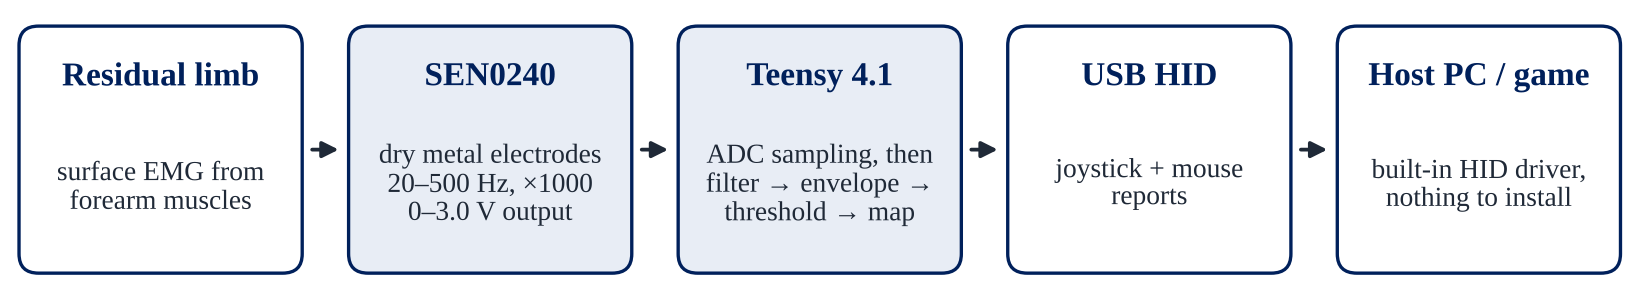
\includegraphics[width=\textwidth]{fig1_system.png}
\caption{MyoElektra signal path, from the sEMG sensor on the residual limb through the Teensy~4.1 to the host as a standard USB HID gamepad.}
\label{fig:system}
\end{figure*}

Levels~0 and~1 rely on basic switches and buttons, so nearly every input requires a physical press. Level~0 includes large press switches, foot pedals and one-handed controllers, which connect through a 3.5~mm jack or USB. Level~1 includes accessible hubs such as the Xbox Adaptive Controller, which has two large buttons and nineteen 3.5~mm jacks, one for each standard controller input, so any switch plugged into it acts as part of a normal controller~\cite{xac}. These hubs have the right output, but every input still depends on a press, which limits users with limb loss on both arms or above the elbow.

Level~2 uses surface electromyography (sEMG), the electrical activity of muscles measured through the skin, but its output usually goes to a proprietary system or app. The Mudra Link reads signals at the wrist to detect finger gestures such as a pinch and, after setup in its app, acts as a Bluetooth mouse and keyboard~\cite{mudra}. The Meta Neural Band reads wrist sEMG but is sold with, and works through, Meta's display glasses~\cite{neuralband}. Both are worn on the wrist and trained on the finger gestures of an intact hand, so neither is designed or tested for a residual limb. Myoelectric prostheses are the opposite case: they are built for amputees, but their sEMG only moves a prosthetic hand. Since the consumer Myo armband was discontinued, researchers report a lack of low-cost, easy-to-use EMG sensors for home use and increasingly build custom EMG hardware for each system~\cite{garske}.

Levels~3 and~4 require surgery. Targeted muscle reinnervation (TMR) transfers the nerves that once controlled the hand onto remaining muscles, such as those of the chest, so that attempting to close the missing hand contracts that muscle; the resulting sEMG gives a prosthetic arm additional, more intuitive control sites~\cite{kuiken}. Intracortical brain--computer interfaces such as Neuralink's implant aim to let people with paralysis control computers with their thoughts, but they require brain surgery and remain in clinical trials~\cite{prime}.

Research systems show what decoded sEMG can do. MyoGestic decodes multiple spared motor dimensions in people with amputation and spinal cord injury~\cite{myogestic}, but it runs on a host computer. Across the products and research reviewed, none reads sEMG from a residual limb and appears to the computer as a standard USB gamepad without drivers or host software, that is, Level~2 input with Level~1 output.

MyoElektra aims to fill this gap. Its goal is a non-invasive, low-cost controller that turns muscle signals from the residual limb into a standard USB human interface device (HID): plugged into any computer, it appears as an ordinary gamepad and mouse, with nothing to install and no gel to apply. Gaming is the primary use case because it demands fast, accurate input, and the same standard output covers menus, browsing and general computer use. This semester's objectives are to (i)~configure a Teensy~4.1 as a USB HID game controller, (ii)~prove that a real muscle signal can trigger a controller input, and (iii)~build and validate a processing and mapping pipeline on simulated EMG. The spring semester moves to real residual-limb signals, physical devices that use controllers such as an RC car or drone, and, if approved, testing with users.

\begin{table}[!t]
\caption{Existing Options for Computer Input After Hand Loss}
\label{tab:ladder}
\centering
\footnotesize
\setlength{\tabcolsep}{3pt}
\renewcommand{\arraystretch}{1.15}
\begin{tabularx}{\columnwidth}{@{}>{\raggedright\arraybackslash}p{1.45cm}>{\raggedright\arraybackslash}X>{\raggedright\arraybackslash}X>{\raggedright\arraybackslash}X@{}}
\toprule
\textbf{Level} & \textbf{Input} & \textbf{Examples} & \textbf{Output} \\
\midrule
0 $\cdot$ Physical & Press or step & Large switches, foot pedals & 3.5~mm jack, USB \\
1 $\cdot$ Adaptive hub & Physical switches & Xbox Adaptive Controller~\cite{xac} & Standard USB controller \\
2 $\cdot$ Surface EMG & Muscle activity on skin & Mudra Link~\cite{mudra}, Meta Neural Band~\cite{neuralband}, prostheses & Bluetooth, glasses, or prosthetic hand \\
3 $\cdot$ Surgical EMG & Reinnervated muscle & TMR prosthetic arms~\cite{kuiken} & Prosthetic arm \\
4 $\cdot$ Brain implant & Cortical signals & Neuralink (trial)~\cite{prime} & Custom software \\
\bottomrule
\end{tabularx}
\end{table}

% ---------------------------------------------------------------------------
\section{Methods}

\subsection{System Architecture}

Fig.~\ref{fig:system} shows the signal path. A single sEMG sensor on the residual limb feeds an analog input of the Teensy~4.1, which filters the signal, extracts an envelope, detects contractions and sends USB HID joystick and mouse reports. Because HID is a standard USB device class with drivers built into common operating systems~\cite{hid}, the host needs nothing installed. The design goals are plug-and-play operation, non-invasive sensing, a parts cost under US\$100, and putting the device on without gel.

\subsection{Hardware Selection}

The Teensy~4.1 was chosen for its native USB device support, including a joystick mode with 32 buttons and 6 axes, a 600~MHz Cortex-M7 with a floating-point unit for real-time filtering, and 18 analog inputs for additional channels~\cite{teensy}. Its pins tolerate only 3.3~V, which constrains the sensor choice.

Table~\ref{tab:sensors} compares the three sensors considered. The Olimex SHIELD-EKG-EMG was excluded because its 40~Hz low-pass filter, designed for electrocardiography (ECG), removes most of the sEMG signal: the spectrum extends to roughly 400~Hz, and most of its power lies between 20 and 200~Hz~\cite{deluca}. The MyoWare~2.0~\cite{myoware} and SEN0240~\cite{sen0240} both cover the sEMG band. The SEN0240 was selected because dry use is its designed configuration, whereas the MyoWare is built around disposable gel pads, and because its 0--3.0~V output stays below the Teensy's 3.3~V limit, while the MyoWare's can reach 5~V. Dry contacts can be more sensitive to motion than gel~\cite{li2020}, although thin dry electrodes have matched clinical electrodes in signal-to-noise ratio~\cite{yamagami2018}; the SEN0240 also accepts gel pads as a fallback. Both electrode types will be tested for signal quality, but dry electrodes are preferred because they fit the plug-and-play goal: the device can be strapped on without skin preparation or replacing gel pads.

\begin{table}[!t]
\caption{sEMG Sensor Comparison}
\label{tab:sensors}
\centering
\footnotesize
\setlength{\tabcolsep}{4pt}
\renewcommand{\arraystretch}{1.15}
\begin{tabular}{@{}llll@{}}
\toprule
 & \textbf{MyoWare 2.0} & \textbf{Olimex shield} & \textbf{SEN0240} \\
\midrule
\textbf{Passband} & 20.8--498.4~Hz & 40~Hz low-pass & 20--500~Hz \\
\textbf{Electrodes} & Snap-on gel pads & Gel pads & Metal dry \\
\textbf{Output} & 0--$V_\mathrm{in}$ ($\leq$5~V) & --- & 0--3.0~V \\
\bottomrule
\end{tabular}
\end{table}

\subsection{Controller Firmware}

Firmware is written in Arduino C++ using PJRC's Teensyduino core and uploaded with arduino-cli. The Teensy is set to the composite ``Serial + Keyboard + Mouse + Joystick'' USB type, so the computer detects one board as four standard devices at once: a serial port for debugging, a keyboard, a mouse and a joystick. So far, simulated inputs have driven mouse reports, moving the cursor on the host. The joystick interface is recognized as a controller (Fig.~\ref{fig:steam}), and hardcoded joystick reports have been tested in a game (Section~\ref{sec:hid}).

\subsection{Planned Signal Processing}
\label{sec:dsp}

The SEN0240 outputs the amplified raw sEMG centered on a 1.5~V reference~\cite{sen0240}. The Teensy will sample it at 2~kHz, more than twice the sensor's 500~Hz upper limit as the Nyquist criterion requires, with margin for the gradual roll-off of the sensor's analog filter. A second-order 20~Hz high-pass filter then removes the 1.5~V offset, movement artifact, and baseline drift~\cite{deluca}. The envelope, which tracks how strongly the muscle is contracting, is the root-mean-square (RMS) of the filtered signal over a 50~ms moving window (Fig.~\ref{fig:pipeline}). A short calibration records each user's resting level and strongest contraction, and the envelope is normalized to that range so that thresholds adapt to each person instead of being fixed.

With one sensor, two contraction strengths can map to two buttons. Two strengths on one sensor have been used to control prostheses since the 1960s, though early systems reported unintended activations when nearby muscles fired at the same time~\cite{dorcas}; this is why the false-trigger test in Section~\ref{sec:testing} includes unrelated motion. When the normalized envelope crosses a soft threshold (initially 15\%), the firmware waits an initial 60~ms to see whether it also crosses a hard threshold (60\%) before committing a button; without this wait, every hard contraction would briefly register as a soft one on its way up. The right wait depends on how quickly a hard contraction rises from the soft to the hard threshold, which will be measured once the sensor arrives: a shorter wait lowers latency but misreads more hard presses as soft. The press is held until the envelope falls 5\% below the soft threshold. This gap, called hysteresis, stops a signal that hovers near a threshold from toggling the button repeatedly. The 50~ms window delays the envelope by about 25~ms, so together with the 60~ms wait, processing alone uses most of the 100~ms latency target.

How well soft and hard contractions can be separated within that latency target sets the number of channels. If they separate reliably, each sensor provides two inputs and fewer sensors are needed; if they overlap, each sensor provides one on/off input and more sensors are added, up to the number of independent muscle sites on the residual limb. Short, held and double contractions can add inputs in either case, but they also add delay, because the firmware must wait to see how long a contraction lasts.

\begin{figure}[!t]
\centering
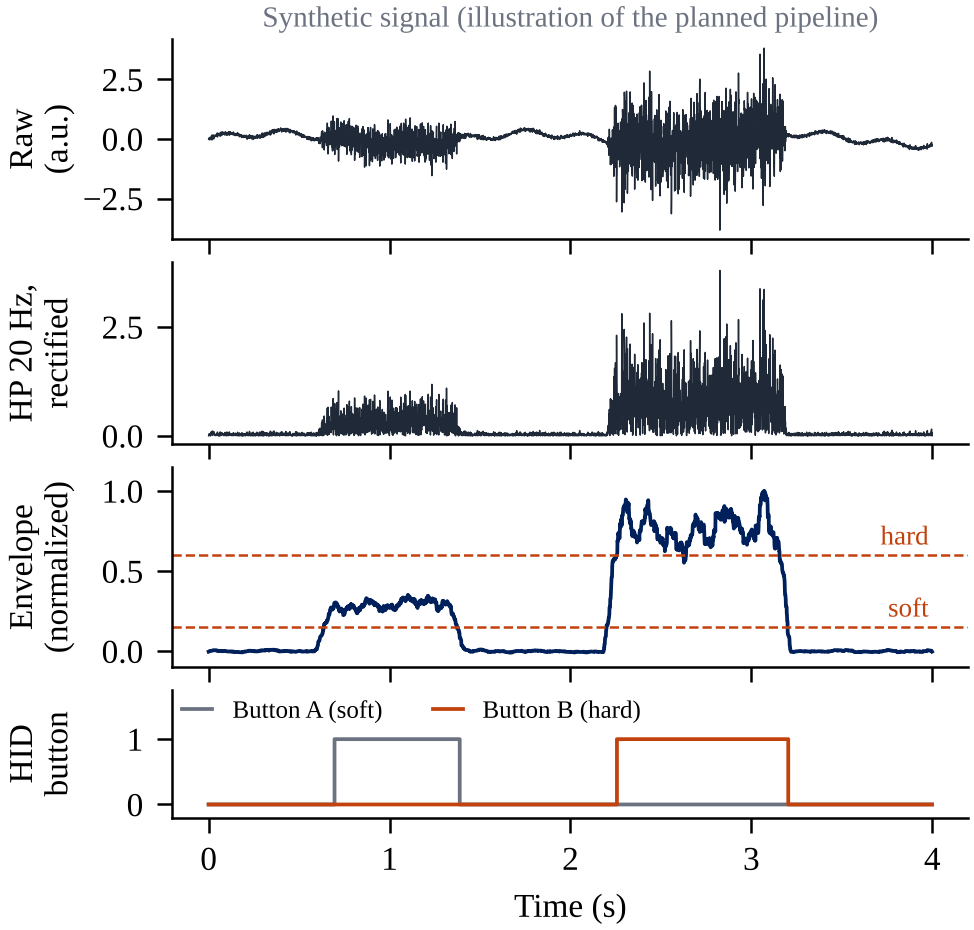
\includegraphics[width=\columnwidth]{fig2_pipeline.png}
\caption{Planned processing chain on a synthetic signal with one soft and one hard contraction plus drift: raw, 20~Hz high-passed (shown rectified), normalized RMS envelope with thresholds, and HID button states. Simulated for illustration; not measured data.}
\label{fig:pipeline}
\end{figure}

\subsection{Staged Testing and Evaluation}
\label{sec:testing}

Testing is staged so that each step adds one new source of error. First, a proof of concept with the SEN0240 on the author's forearm uses a simple threshold to show that a real contraction can press a controller button; this confirms the hardware path but is not tuned. Second, a synthetic signal, band-limited (20--450~Hz) Gaussian noise whose amplitude follows programmed contractions plus low-frequency drift, is run through the firmware on the Teensy itself, stored in its flash memory or streamed over USB serial. Because the timing and strength of every contraction are known exactly, this step measures latency and accuracy against ground truth and verifies the firmware, timing and USB output. Third, public sEMG recordings, matched to the 2~kHz sampling rate and normalized as in Section~\ref{sec:dsp}, provide real signals with natural noise and variation for building and tuning the processing. Finally, development moves to the SEN0240 on the author's forearm. If a stage fails after the previous one passed, the fault lies in what that stage added: the processing at the third stage, or the sensor, electrodes or placement at the fourth. Passing on synthetic data does not guarantee that thresholds and window lengths transfer to real signals, which is why they are tuned on recorded data.

Three metrics define success. End-to-end latency, from EMG onset to the USB report, timestamped on the Teensy, must be at most 100~ms, consistent with the 100--125~ms optimal controller delay reported for myoelectric prostheses~\cite{farrell}. Gesture accuracy, the share of cued gestures mapped to the correct input, must be at least 95\%, and false triggers at rest or during unrelated motion must stay below one per minute. Before any on-body test, isolation and skin checks will follow IEC 60601-2-40~\cite{iec}.

% ---------------------------------------------------------------------------
\section{Results (Partial)}

\subsection{Review of Existing Solutions}

The review covered consumer accessibility products, sEMG wearables, myoelectric prostheses, surgical and implanted interfaces, and research and hobby EMG systems (Table~\ref{tab:ladder}). Across the products and research reviewed, none combines residual-limb sEMG input with standard controller output. Prices range from about US\$100 for the Xbox Adaptive Controller~\cite{xac} to US\$499 for the Mudra Link~\cite{mudra} and US\$799 for the Meta Neural Band bundle~\cite{neuralband}. Gaming matters even at Level~4: Neuralink's first trial participant used his implant to play chess and, on his own, \textit{Civilization~VI}, a game he had previously needed help to play~\cite{popsci}. This suggests that regaining access to games is a real priority for people with limited hand function, and MyoElektra aims to meet it without surgery.

\subsection{Components and Cost}

The selected parts cost about US\$91 before shipping (Teensy~4.1, US\$41.50~\cite{amazon}; SEN0240, US\$49.50~\cite{digikey}), well below the US\$499--799 of current EMG wearables. The SEN0240 has been ordered, and on-body work begins once it arrives.

\begin{figure}[!t]
\centering
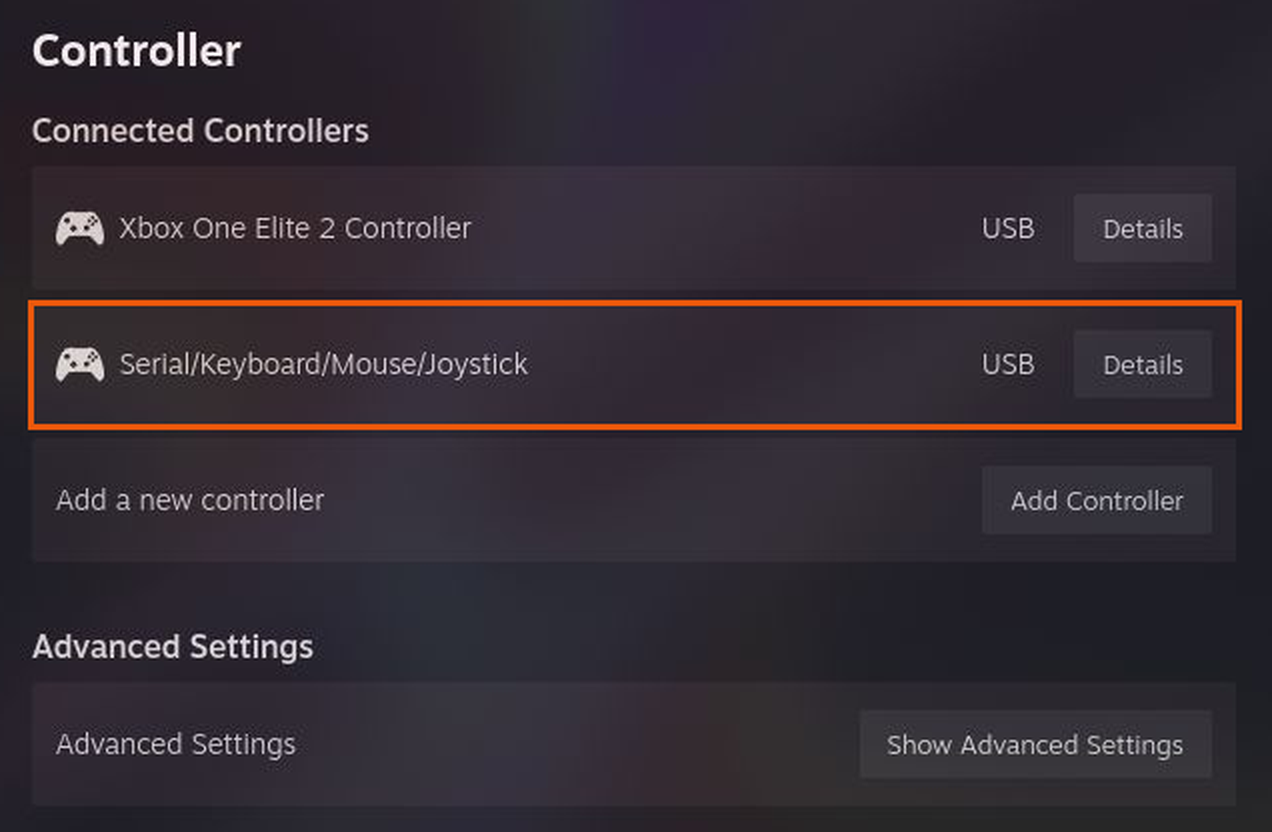
\includegraphics[width=\columnwidth]{fig3_steam.png}
\caption{Steam controller settings showing the Teensy~4.1 (outlined) enumerated as a USB HID controller, with no driver or application installed.}
\label{fig:steam}
\end{figure}

\subsection{USB HID Enumeration}
\label{sec:hid}

The preliminary research and the controller interface are complete. The Teensy~4.1 enumerates as a composite USB device. Steam, a widely used platform for buying and launching PC games, lists it as a connected controller, ``Serial/Keyboard/Mouse/Joystick,'' next to a commercial Xbox controller, with no driver or application installed (Fig.~\ref{fig:steam}). In \textit{Forza Horizon~6}, a racing game, joystick reports from the Teensy steered the car left and right, accelerated and braked. These inputs were hardcoded in firmware rather than driven by EMG; no EMG results exist yet, and they are the focus of the remaining work.

% ---------------------------------------------------------------------------
\section{Discussion (Partial)}

The working controller interface shows that the output side of the gap can be met with commodity hardware: unlike research EMG interfaces that decode on a host computer~\cite{myogestic}, the microcontroller itself appears as a standard controller, and an unmodified commercial game accepted its inputs. What remains unproven is the input side, turning residual-limb sEMG into those same reports.

The main risk is input quality. Dry electrodes showed weaker motion rejection than gel electrodes during walking~\cite{li2020}, so seated use, the 20~Hz high-pass filter, the false-trigger test and the gel fallback are the planned mitigations. The staged testing in Section~\ref{sec:testing} isolates this risk: if the pipeline works on synthetic signals and public recordings but fails with the SEN0240, the fault lies in the sensor or its placement rather than the firmware. The channel count stays open until soft and hard contractions are tested on the SEN0240 (Section~\ref{sec:dsp}). Residual forearm muscles still produce usable EMG for imagined hand movements, with accuracy increasing with the amount of forearm remaining~\cite{atzori}. Because people with limited movement choose very different gestures for the same command~\cite{yamagami2023}, each user will choose which muscle and contraction maps to each button.

Next steps follow the staged plan in Section~\ref{sec:testing}: an EMG proof of concept once the sensor arrives, then the simulated signal source, the processing and mapping pipeline, and tests on public recordings. The minimum goal for the fall semester is for simulated EMG to pass through the full pipeline and control a game.

% ---------------------------------------------------------------------------
\section*{Acknowledgment}

The author thanks Prof.~Jose Moreto for mentorship and feedback throughout the ELEC~594 capstone. Claude (Anthropic) was used to assist with the literature search, drafting and editing of the text. The author declares no conflicts of interest.

\section*{CRediT Author Statement}

\textbf{Alex Smith:} Conceptualization, Methodology, Investigation, Software, Validation, Visualization, Writing -- original draft, Writing -- review \& editing.

% ---------------------------------------------------------------------------
\begin{thebibliography}{99}

\bibitem{xac}
Microsoft, ``Xbox Adaptive Controller,'' Microsoft Store. Accessed: Oct. 23, 2026. [Online]. Available: \url{https://www.microsoft.com/en-us/d/xbox-adaptive-controller/8nsdbhz1n3d8}

\bibitem{mudra}
Wearable Devices Ltd., ``Mudra Link.'' Accessed: Oct. 23, 2026. [Online]. Available: \url{https://mudra-band.com/products/mudra-link}

\bibitem{neuralband}
Meta, ``Meta Neural Band.'' Accessed: Oct. 23, 2026. [Online]. Available: \url{https://www.meta.com/ai-glasses/accessories/neural-band/}

\bibitem{garske}
C.~A. Garske, M.~Dyson, S.~Dupan, and K.~Nazarpour, ``Perception of game-based rehabilitation in upper limb prosthetic training: Survey of users and researchers,'' \textit{JMIR Serious Games}, vol.~9, no.~1, Art. no. e23710, 2021, doi: 10.2196/23710.

\bibitem{kuiken}
T.~A. Kuiken \textit{et al.}, ``Targeted muscle reinnervation for real-time myoelectric control of multifunction artificial arms,'' \textit{JAMA}, vol.~301, no.~6, pp.~619--628, 2009, doi: 10.1001/jama.2009.116.

\bibitem{prime}
Neuralink, ``Precise Robotically IMplanted Brain-Computer InterfacE (PRIME),'' ClinicalTrials.gov, NCT06429735. Accessed: Oct. 23, 2026. [Online]. Available: \url{https://clinicaltrials.gov/study/NCT06429735}

\bibitem{myogestic}
R.~C. S\^{\i}mpetru \textit{et al.}, ``MyoGestic: EMG interfacing framework for decoding multiple spared motor dimensions in individuals with neural lesions,'' \textit{Sci. Adv.}, vol.~11, no.~15, Art. no. eads9150, 2025, doi: 10.1126/sciadv.ads9150.

\bibitem{hid}
USB Implementers Forum, \textit{Device Class Definition for Human Interface Devices (HID)}, ver.~1.11, 2001.

\bibitem{teensy}
PJRC, ``Teensy 4.1 development board.'' Accessed: Oct. 23, 2026. [Online]. Available: \url{https://www.pjrc.com/store/teensy41.html}

\bibitem{deluca}
C.~J. De~Luca, L.~D. Gilmore, M.~Kuznetsov, and S.~H. Roy, ``Filtering the surface EMG signal: Movement artifact and baseline noise contamination,'' \textit{J. Biomech.}, vol.~43, no.~8, pp.~1573--1579, 2010, doi: 10.1016/j.jbiomech.2010.01.027.

\bibitem{myoware}
SparkFun Electronics, ``Getting started with the MyoWare 2.0 muscle sensor ecosystem.'' Accessed: Oct. 23, 2026. [Online]. Available: \url{https://learn.sparkfun.com/tutorials/getting-started-with-the-myoware-20-muscle-sensor-ecosystem}

\bibitem{sen0240}
DFRobot, ``Gravity: Analog EMG sensor by OYMotion (SEN0240).'' Accessed: Oct. 23, 2026. [Online]. Available: \url{https://wiki.dfrobot.com/SEN0240}

\bibitem{li2020}
J.~Li, P.~Wang, and H.~J. Huang, ``Dry epidermal electrodes can provide long-term high fidelity electromyography for limited dynamic lower limb movements,'' \textit{Sensors}, vol.~20, no.~17, Art. no. 4848, 2020, doi: 10.3390/s20174848.

\bibitem{yamagami2018}
M.~Yamagami \textit{et al.}, ``Assessment of dry epidermal electrodes for long-term electromyography measurements,'' \textit{Sensors}, vol.~18, no.~4, Art. no. 1269, 2018, doi: 10.3390/s18041269.

\bibitem{dorcas}
D.~S. Dorcas and R.~N. Scott, ``A three-state myo-electric control,'' \textit{Med. Biol. Eng.}, vol.~4, no.~4, pp.~367--370, 1966, doi: 10.1007/BF02476154.

\bibitem{farrell}
T.~R. Farrell and R.~F. Weir, ``The optimal controller delay for myoelectric prostheses,'' \textit{IEEE Trans. Neural Syst. Rehabil. Eng.}, vol.~15, no.~1, pp.~111--118, Mar. 2007, doi: 10.1109/TNSRE.2007.891391.

\bibitem{iec}
\textit{Medical Electrical Equipment---Part 2-40: Particular Requirements for the Basic Safety and Essential Performance of Electromyographs and Evoked Response Equipment}, IEC 60601-2-40:2024, 2024.

\bibitem{popsci}
A.~Paul, ``Neuralink shows first human patient using brain implant to play online chess,'' \textit{Popular Science}, Mar. 21, 2024. Accessed: Oct. 23, 2026. [Online]. Available: \url{https://www.popsci.com/technology/neuralink-first-human-video/}

\bibitem{amazon}
``PJRC Teensy 4.1 with pins,'' Amazon.com. Accessed: Oct. 23, 2026. [Online]. Available: \url{https://www.amazon.com/PJRC-Teensy-4-1-with-Pins/dp/B08CTM3279}

\bibitem{digikey}
DigiKey, ``DFRobot SEN0240.'' Accessed: Oct. 23, 2026. [Online]. Available: \url{https://www.digikey.com/en/products/detail/dfrobot/SEN0240/8019061}

\bibitem{atzori}
M.~Atzori \textit{et al.}, ``Effect of clinical parameters on the control of myoelectric robotic prosthetic hands,'' \textit{J. Rehabil. Res. Dev.}, vol.~53, no.~3, pp.~345--358, 2016, doi: 10.1682/JRRD.2014.09.0218.

\bibitem{yamagami2023}
M.~Yamagami, A.~A. Portnova-Fahreeva, J.~Kong, J.~O. Wobbrock, and J.~Mankoff, ``How do people with limited movement personalize upper-body gestures? Considerations for the design of personalized and accessible gesture interfaces,'' in \textit{Proc. 25th Int. ACM SIGACCESS Conf. Comput. Accessibility (ASSETS)}, New York, NY, USA, 2023, doi: 10.1145/3597638.3608430.

\end{thebibliography}

\end{document}
